\documentclass{article}
\usepackage[color=red]{todonotes}
\usepackage[utf8]{inputenc}
\usepackage[T1]{fontenc}
\usepackage{tikz}
\usetikzlibrary{bayesnet}
\usepackage{amsmath}
\usepackage{xcolor}

\newcommand{\program}{\rho}

\newcommand{\inputs}{X}

\newcommand{\outputs}{Y}

\begin{document}

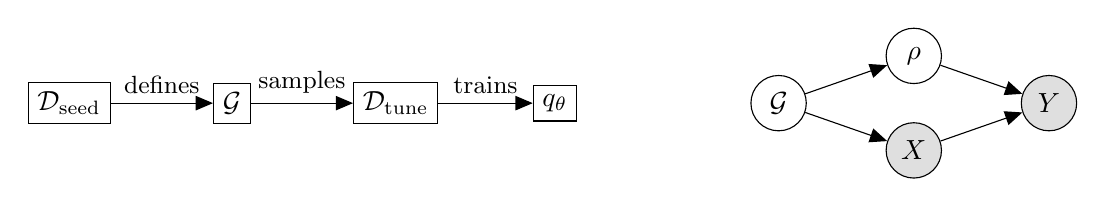
\begin{tikzpicture}
    \node[draw] (s) {$\mathcal{D}_\text{seed}$};
    \node[draw, right=of s, xshift=0.3cm] (g2) {$\mathcal{G}$};
    \draw[->] (s) -- node [above,midway] {\small defines} (g2);
    \node[draw, right=of g2, xshift=0.3cm](t) {$\mathcal{D}_\text{tune}$};
    \draw[->] (g2) -- node [above,midway] {\small samples} (t);
    \node[draw, right=of t, xshift=0.2cm] (lm) {$q_\theta$};
    \draw[->] (t) -- node [above,midway] {\small trains} (lm);
        
    \node[latent, right=of lm, xshift=1.2cm] (g) {$\mathcal{G}$} ; %
    \node[latent, right=of g, yshift=0.6cm] (p){$\program$};
    \node[obs, right=of g, yshift=-0.6cm] (x){$\inputs$};
    \node[obs, right=of p, yshift=-0.6cm] (y){$\outputs$};
    \edge[->] {g} {p};
    \edge[->] {g} {x};
    \edge[->] {p,x} {y};
\end{tikzpicture}

\end{document}